\chapter{数据获取与预处理}\thispagestyle{fancy}
本章将从系统使用的数据集,情感词典和预处理流程三方面进行介绍。
\section{数据集}
为了评估数据模型的准确性以及训练模型以便展示等目的,本文针对语句级任务获取了以下数据集。
\begin{center}
\begin{longtabu} to \textwidth {|X[m]|X[4]|}
\toprule
名称 & NLPCC 2014 SCDL数据集中文\\
\hline
\hline
数据总数 & 12500条\\
\hline
数据集大小 & 4.4MB\\
\hline
官方测试集数据总数 & 中文2500条\\
\hline
语言 & 中文\\
\hline
比例 & 正向:负向 6250:6250\\
\hline
测试集比例 & 正向:负向 1250:1250\\
\hline
词数最大值 & 中文 800词数量级\\
\hline
99\%词数 & 中文 200词数量级\\
\hline
情感分类准确度 & 不够准确\\
\hline
语句特点 & 语句较为口语化,有广告等中性语句\\
\hline
获取方式 & \url{http://tcci.ccf.org.cn/conference/2014/pages/page04_sam.html}\newline (Accessed at: 5/21/2017)\\
\hline
主要用途 & 评估模型性能\\
\hline
\hline
词频统计 & -\newline - 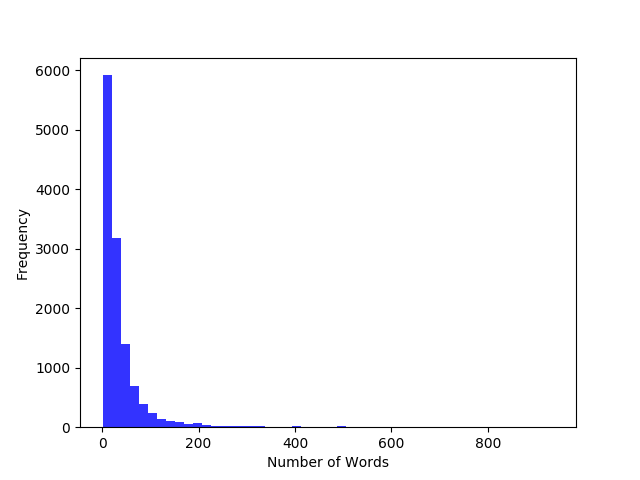
\includegraphics[width=0.75\textwidth, height=0.5\textwidth]{graphic/wordsnum_nlpcc_zh.png}\\
\hline 
\hline
名称 & NLPCC 2014 SCDL数据集英文\\
\hline
\hline
数据总数 & 12485条\\
\hline
数据集大小 & 9.0MB\\
\hline
官方测试集数据总数 & 2500条\\
\hline
语言 & 英文\\
\hline
比例 & 正向:负向 6237:6248\\
\hline
测试集比例 & 正向:负向 1250:1250\\
\hline
词数最大值 & 6000词数量级\\
\hline
99\%词数 & 1000词数量级\\
\hline
情感分类准确度 & 较为准确\\
\hline
语句特点 & 词汇较丰富,部分评论中单词没有以空格或其它分隔符分开\\
\hline
获取方式 & \url{http://tcci.ccf.org.cn/conference/2014/pages/page04_sam.html}\newline (Accessed at: 5/21/2017)\\
\hline
主要用途 & 评估模型性能\\
\hline
词频统计 & -\newline - 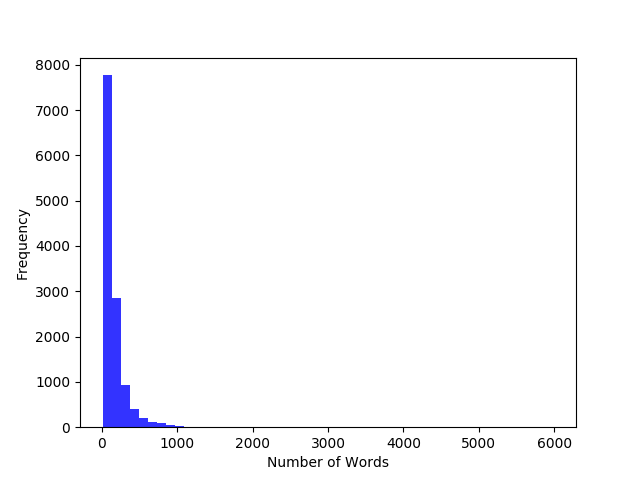
\includegraphics[width=0.75\textwidth, height=0.5\textwidth]{graphic/wordsnum_nlpcc_en.png}\\
\hline 
\hline
名称 & 携程数据集\\
\hline
\hline
数据总数 & 1710000条\\
\hline
数据集大小 & 39.2MB\\
\hline
语言 & 中文\\
\hline
比例 & 正向:中性:负向=57000:57000:57000\\
\hline
测试方法 & 5 fold\\
\hline
词数最大值 & 1750词数量级\\
\hline
99\%词数 & 250词数量级\\
\hline
情感分类准确度 & 不够准确\\
\hline
语句特点 & 语句较为口语化\\
\hline
获取方式 & 通过selenium模拟浏览器爬取\\
\hline
主要用途 & 模型展示\\
\hline
词频统计 & -\newline - 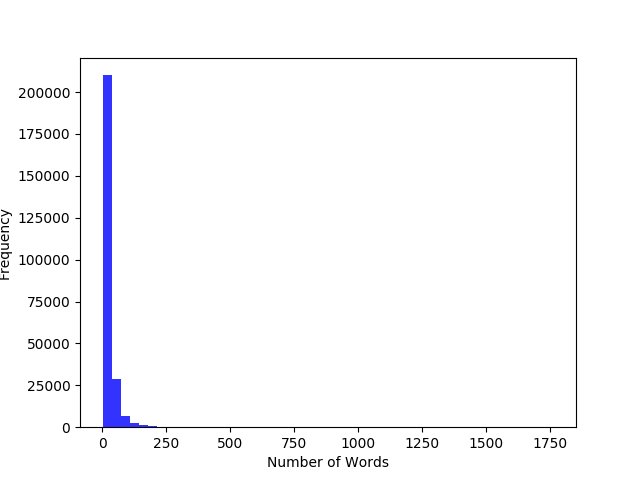
\includegraphics[width=0.75\textwidth, height=0.5\textwidth]{graphic/wordsnum_xiecheng.png}\\
\bottomrule
\caption{数据集一览}
\end{longtabu}
\end{center} 


\paragraph*{备注1\ 99\%词数} 
本文中数据集普遍存在部分过长评论,这些过长评论的词数往往是数据集中99\%的语句的词数的4-8倍。在实际训练CNNPL网络的过程中,为这些过长的语句额外训练参数会大幅增加模型的时空复杂度,因此本文选取99\%语句的词数作为CNNPL网络处理的词数,超过该词数的文本将被截断。同时,这也是为了训练CNNPL网络仅使用文本前半段判断文本整体情感极性的能力。


\paragraph*{备注2\ 携程数据集获取过程}
由于NLPCC 2014的SCDL数据集样本容量较少,本文通过selenium模拟浏览器爬取携程网站中国内酒店带有评分的评论388067条用于展示和评估。由于携程酒店的评分是5分制,根据人们在购物网站评分时的心态,我们将满分5分的评论定为正向评价,严格小于4分的评论定为负向评价,其余的定为中性评价,得到正向评价193138条,中性评价137604条,负向评价57325条。为了平衡数据集,避免神经网络模型对特定标签产生偏置,我们随机抽取其中正向评价,中性评价,负向评价各57000条,组成携程数据集。


\section{情感词典} \label{sec:emotionset}
由于知识模型可以同时支持中/英文分析,故情感词典主要由以下两种语言共六个词典组成。
\subsection{中文情感词典}
\begin{enumerate}
\item Hownet(知网)情感词典\cite{hownet}:语言为中英双语。该词典为董振东和董强建立的情感分析用语集,包括主张词语,正面/负面情感词语,正面/负面评价词语,程度级别词语,并为程度级别词语划分强度等级。但其中有一些不常使用的词语,如"噲","媢","媢嫉","忺","安","巴"等在正面情感词典中出现的词。另外词语可能以短语形式出现,如"越...越...","abandon oneself to despaire"等。
\item NTUSD台湾大学情感词典\cite{ntusd}:台湾大学自然语言处理实验室提供的情感词典,包括正面词汇2810个和负面词汇8276个,极性划分较为准确,且包含各种词性,如“一下子爆发”,“一下子爆发的一连串,“一巴掌”。
\item DUTIR情感词汇本体库\cite{dutir}:大连理工大学信息检索研究室整理和标注的中文情感词库,具有词性,情感分类,强度,极性和辅助情感分类,强度,极性等特征,划分详细。包含各种词性,但以成语和俗语为主体。
\end{enumerate}
\subsection{英文情感词典}
\begin{enumerate}
\item SentiWordNet\cite{sentiwordnet} \cite{sentiwordnet3}:基于WordNet3.0,具有语义,正向评分PosScore和负向评分NegScore等信息,本文中取PosScore-NegScore之差作为其分数。
\item Opinion Lexicon:Bing Liu等\cite{huliu2004a} \cite{huliu05a} 整理的极性情感词典,仅包含单词本身,不包含短语,但包括单词的各种变形形式。
\item 匹兹堡大学MPQA主观性词典\cite{mpqa}:是MPQA(Multi-Perspective Question Answering,多方面问答)系统所用到的词典,具有情绪词,词性,情感强弱等词汇信息。
\end{enumerate}

\section{数据预处理}
在有监督学习的过程中,如何选择特征,选择何种特征将对训练结果和泛化性产生极大的影响。实际环境中,文本往往含有不规范的表达方式及符号,因此有必要对文本进行一系列预处理。本文根据现有文献的经验,分析目前流行的文本预处理工具后,根据不同语言选择不同预处理工具,得出了下列文本预处理的流程。

\subsection{基本流程}
如图\ref{fig:preprocessing} 表示了整个文本情感分类系统的基本预处理流程,对所有模型,都需要对文本进行转换编码,去除非法字符,化繁为简和短句切分,分词这些预处理工作。其中分词则是重中之重,会对所有模型的准确率产生很大影响。同时,机器学习模型在训练模式下需要生成词汇表,训练待编码特征对应的编码,并将语句各特征抽取出来以备训练或预测情感极性使用。

\begin{figure}[!htbp]
\begin{center}
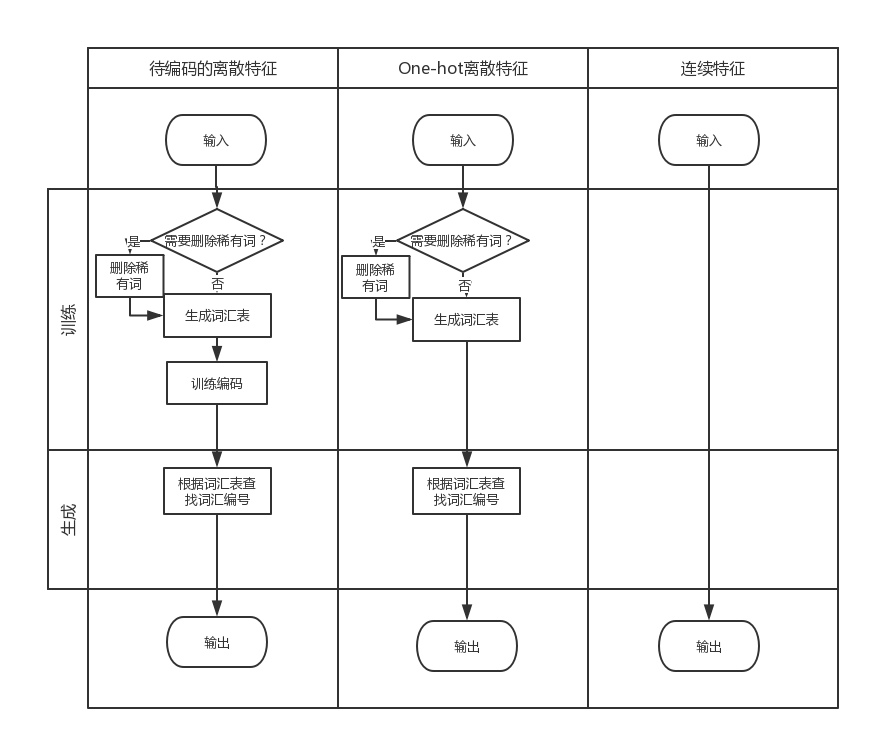
\includegraphics[width=\textwidth]{graphic/prepocessing.png}
\caption{数据预处理基本流程图 \label{fig:preprocessing}}
\end{center}
\end{figure}

\subsection{分词}
\subsubsection{中文}
本文从携程数据集和NLPCC中文任务中随机抽取15条语句,使用相同的用户自定义词典,对比了三种分词工具thulac,ansj,jieba的精准分词性能,结果如\nameref{appendix:parsercompare}所示。由于ansj工具的实体识别能力最强,故选择ansj工具。\par
ansj是由孙健实现的,具有分词,标注词性,实体识别,关键词抽取及新词发现功能的java中文分词工具。该工具使用隐马尔科夫模型进行语义消歧,使用Hash和高度优化Trie树进行词典匹配,并使用条件随机场模型(CRF)进行新词发现。\cite{ansjwiki} 本文主要使用到其分词,标注词性,实体识别及新词发现功能。\par
对于新词发现功能,本文主要学习输入语料中的新词,然后对这些新词进行手工过滤,加入情感词典以及ansj用户自定义词典。其中用户自定义词典人工过滤8430条,过滤得到3137条词条,157条情感词典词条。
\subsubsection{英文}
与没有分隔符的中文相比,英文短句中的单词之间由空格作为分隔符,更易于分隔,因而英文的分词难度远远小于中文分词。但由于英文文本中存在标点符号和不规则语用现象,本文选择使用Stanford CoreNLP工具进行分词。同时,这一步也是为了知识模型生成语法树做准备。\par
Stanford CoreNLP工具是由斯坦福大学自然语言处理实验室研发的\cite{corenlp},可以处理分句(ssplit),分词(tokenize),词性标注(POS),词干化(lemma),命名实体分析(NER),语法树分析(parse),短句情感分析(sentiment)和词语分析(natlog)等多种任务的工具集。本文中主要用到其中的分词,分句,词性标注,词干化,语法树分析等功能。\par
该工具集基于Java,由管道(Pipeline)将各子工具连接,从而方便地复用了各子工具。\par
以下代码为本文系统JAVA部分调用Stanford CoreNLP工具的代码:\par
\lstset{language=java}
\begin{lstlisting}
new StanfordCoreNLP(
  PropertiesUtils.asProperties("annotators",
    "tokenize,ssplit,truecase,pos," + 
    "lemma,ner,parse,sentiment",
    "tokenize.language", "en"));
\end{lstlisting}

图\ref{fig:corenlpf1} \cite{corenlp} 是Stanford CoreNLP 整体流程的说明,如图,文本被转化为Annotation对象然后输入各子工具集,各子工具集可选,但内部存在依赖顺序。\par
图\ref{fig:corenlpf2} \cite{corenlp} 则是Stanford CoreNLP2014年各子工具集的语言支持情况,可以看到,该工具集可以处理多种语言,其中对英文支持最为全面准确。同时,该工具集支持中文的句法分析,满足知识模型需求。

\begin{figure}[!htbp]
\begin{center}
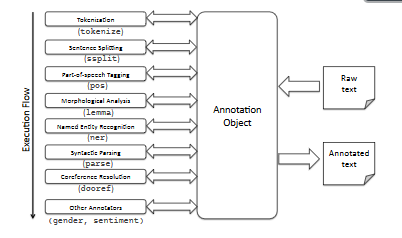
\includegraphics[width=\textwidth]{graphic/stanfordcorenlpf1.PNG}
\caption{Stanford CoreNLP整体流程图 \label{fig:corenlpf1}}
\end{center}
\end{figure}


\begin{figure}[!htbp]
\begin{center}
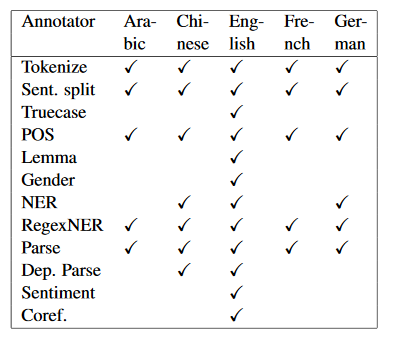
\includegraphics[width=0.6\textwidth]{graphic/stanfordcorenlpf2.PNG}
\caption{Stanford CoreNLP语言支持情况 \label{fig:corenlpf2}}
\end{center}
\end{figure}


\subsection{输入特征}
为了便于拓展模型和系统,本文将特征分为三类:\par
\begin{enumerate}
\item 待编码的离散特征,为了便于表示,简称为Emb Feature。
\item One-hot离散特征: Onehot Feature。
\item 连续特征: C Feature。
\end{enumerate}
\par
三种特征各自有不同的处理方式。同时,对于某些离散特征,本文会删除词频较低的词汇,以提高模型拓展性,简称为 Del Feature,详细分析请见\ref{sec:rareword}。
\subsubsection{特征处理}
按照不同特征的类别,处理方式见图\ref{fig:featureprocessing},其中One-hot特征和Emb特征都需要转为编号,Emb特征需要进一步训练并转化为编码。生成阶段将Emb特征编号转化为编码与训练模型具体处理方式有关,因此本系统不将之列入预处理流程。
\begin{figure}[!htbp]
\begin{center}
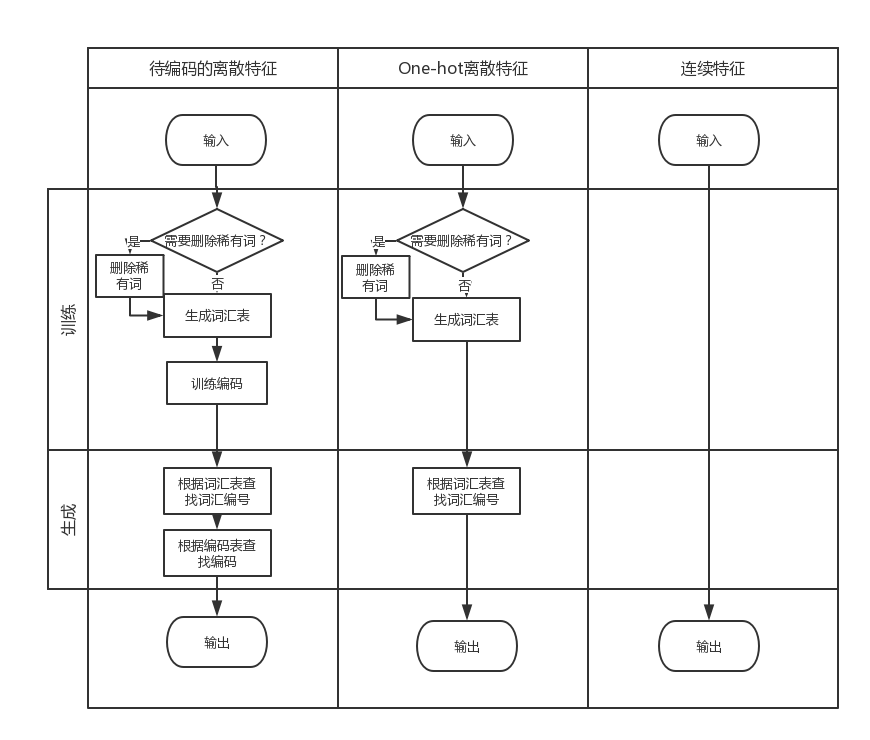
\includegraphics[width=\textwidth]{graphic/featurepocessing.png}
\caption{数据预处理基本流程图 \label{fig:featureprocessing}}
\end{center}
\end{figure}
\subsubsection{特征选择}
\begin{center}
\begin{longtabu} to \textwidth{X|X|X[3]|X[3]} 
\toprule
& 层级 & 中文 & 英文\\
\hline
知识模型 & 语句级 & 词汇(C) & 词性还原化词汇(C)\\
\hline
NOLSTM模型 & 语句级 & 词汇编码(Emb,Del),词性(Onehot) & 词汇编码(Emb,Del),词干编码(Emb,Del),词性(Onehot)\\
\hline
CLSTM模型 & 语句级 & 词汇编码(Emb,Del),词性(Onehot) & 词汇编码(Emb,Del),词干编码(Emb,Del),词性(Onehot)\\
\bottomrule
\caption{各模型特征及类型}
\end{longtabu}
\end{center}

\subsection{稀有词删除}
该步骤统计某特征在训练集中出现频率,之后将出现频率小于规定的最低频度的特征置换为一个特殊词"RAREWORD"。对于词性为nt(机构团体), ns(地名), nr(人名), nz(其它专有名词)的单词所对应的特征,规定的最低频度通常大于全局最低频度,以删除专有名词,尽量减少这类无用词的影响。


本文中所用到的频率限制为:中文全局最低频率为7,专有名词最低频率限制为12。英文全局最低频率为12,由于英文文本的词性标注方式与中文文本不同,书名,机构名,人名等往往被识别为名词,因此很难识别英文文本中专有名词和普通名词的差别,故不设置特殊的专有名词最低频率。

\subsection{英文词性还原及词干化}
英文中动词往往具有多种时态,如过去式,现在进行时,一般现在时等,如got,gotten,get,getting,gets。同时,形容词和副词也常常具有同样的词干,如happy, happily。这些单词虽然形态不同,却具有语义上的联系,因此,有必要对单词进行词性还原和词干提取,以发现其内部隐含的语义联系。\par
本文使用Stanford CoreNLP对单词进行词性还原,之后再使用nltk Snowball Stemmer进行词干化,以此作为英文模型的输入特征。相关测试见\nameref{appendix:lemmacompare}。

\subsection{特征生成详细流程}
本章详细介绍并举例说明模型的特征生成过程。其中,中文英文的生成流程略有差别。
\subsubsection{知识模型}
知识模型接受的输入为单词或者经过了词性还原的单词。当处理中文时,如图\ref{fig:preprocesskzh},本文首先将进行编码转换工作,并将可能存在的繁体中文文本转化为简体中文,然后,本文使用ansj工具进行分词,将分词后的文本输入知识模型。而处理英文时,由于英文有较多时态变化,本文选择对英文单词做词性还原操作。如图\ref{fig:preprocessken},本文首先进行编码转换,同时删除不应该出现在英文文本中的字符如汉语全角标点符号等,接着,本文使用Stanford CoreNLP工具进行分词,分词后的结果经过单词小写化处理后,还需要再使用Stanford CoreNLP进行词性还原,最后,词性还原后的单词才能输入知识模型进行分析。


\begin{figure}[!htbp]
\begin{center}
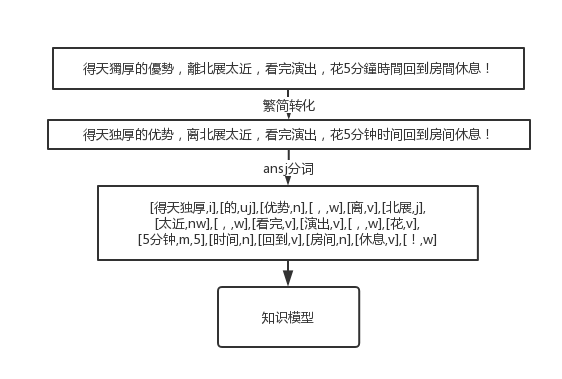
\includegraphics[width=\textwidth]{graphic/preprocesskzh.png}
\caption{知识模型中文特征生成流程图 \label{fig:preprocesskzh}}
\end{center}
\end{figure}


\begin{figure}[!htbp]
\begin{center}
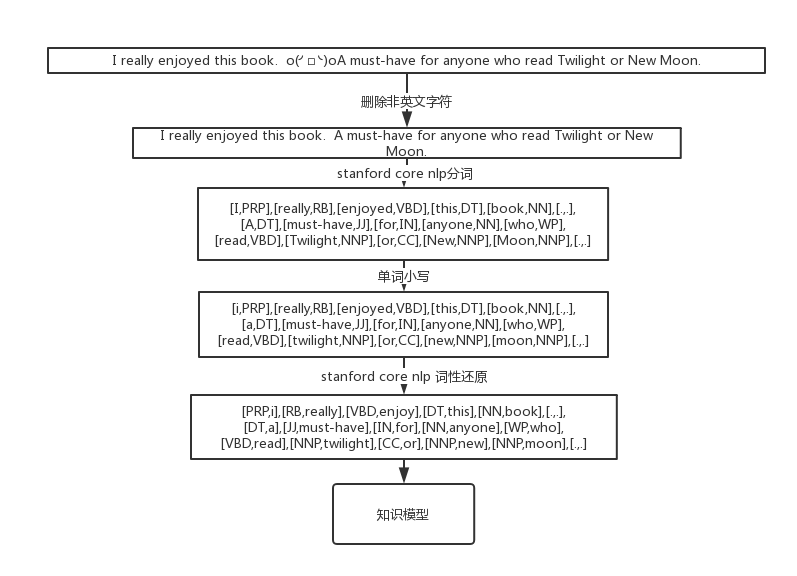
\includegraphics[width=\textwidth]{graphic/preprocessken.png}
\caption{知识模型英文特征生成流程图 \label{fig:preprocessken}}
\end{center}
\end{figure}

\subsubsection{CNNPL模型}
神经网络模型接受的参数为文本转化成的固定长度的向量,其中CNNPL模型接受一组固定长度的向量,而CNNLSTMPL接受多组固定长度的向量直到序列被遍历完毕。本节将分别介绍CNNPL模型的中英文处理方式。


由于神经网络模型一次只能接受固定长度的向量作为参数,本文中CNNPL模型只取前半段文本中的词汇进行分析,定义CNNPL模型能处理的最大词汇数目为处理长度。如图\ref{fig:preprocessczh},在中文下,经过编码转换,分词工作后,本文删除词汇本身中的稀有词,并为词汇和词性编号,使用word2vec中的Continuous Skip-Gram模型\cite{mikolov2013b}将处理长度内的词汇转换为固定长度的向量,并将词性转化为onehot向量,最后,将二者拼接组成输入特征矩阵。


如图\ref{fig:preprocesscen},在英文下,经过删除非英文字符,小写转换,分词,词性还原工作后,本文使用nltk工具包中的snowball stemmer进行词根化,接着本文分别删除词汇本身和词根中的稀有词,为词汇,词根和词性编号,将处理长度内的词汇和词根都转换为固定长度的向量,最后将二者与词性onehot向量进行拼接。


\begin{figure}[!htbp]
\begin{center}
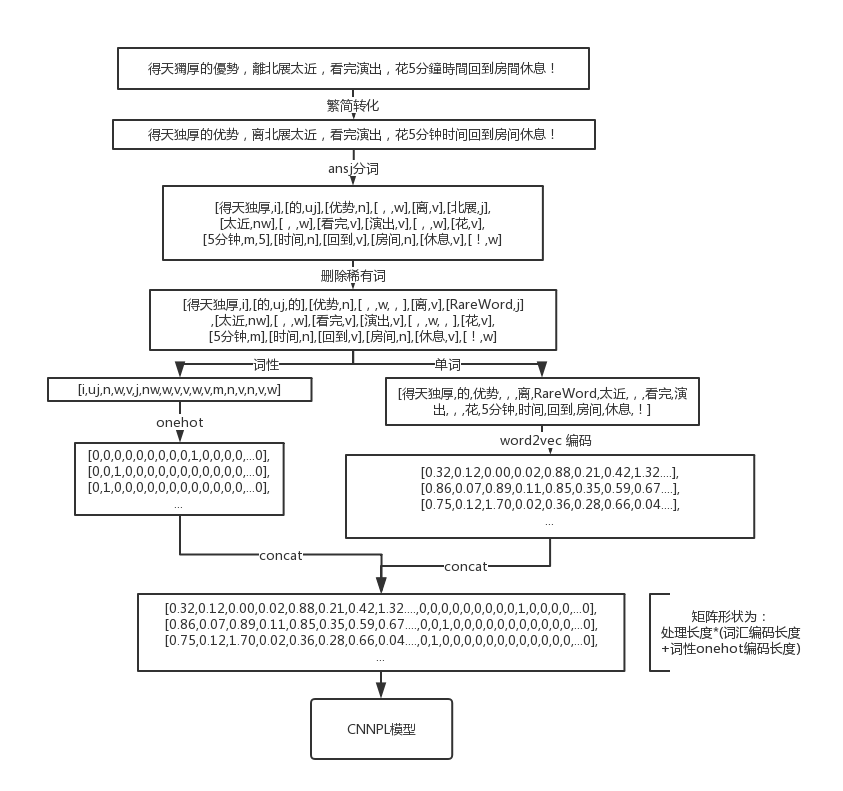
\includegraphics[width=\textwidth]{graphic/preprocessczh.png}
\caption{CNNPL模型中文特征生成流程图 \label{fig:preprocessczh}}
\end{center}
\end{figure}


\begin{figure}[!htbp]
\begin{center}
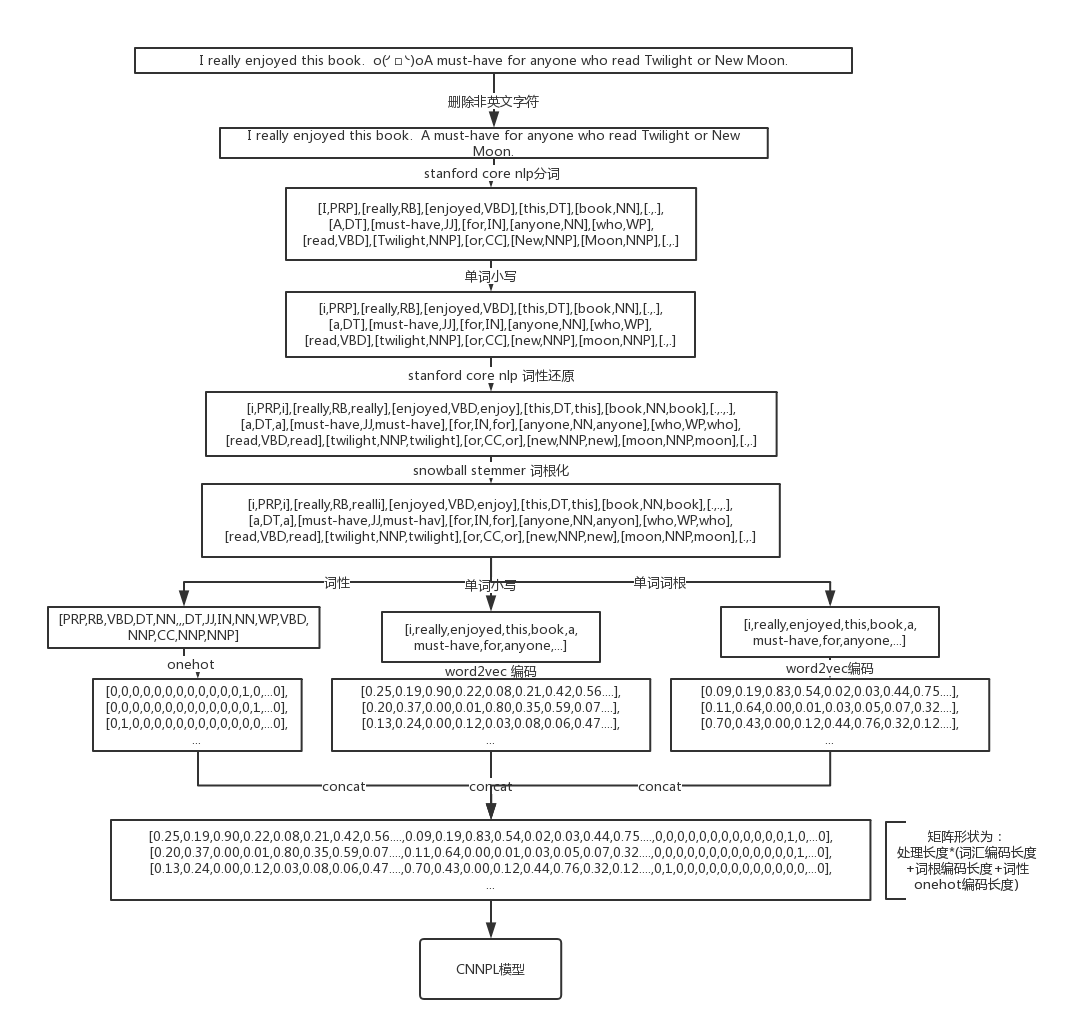
\includegraphics[width=\textwidth]{graphic/preprocesscen.png}
\caption{CNNPL模型英文特征生成流程图 \label{fig:preprocesscen}}
\end{center}
\end{figure}

\subsubsection{CNNLSTMPL模型}
作为循环神经网络,CNNLSTMPL模型需要进行反复迭代。本文将在迭代的某一步中,CNNLSTMPL能处理的最大词汇数目定为处理长度,将此时开始处理的第一个词的位置称为起点。如图\ref{fig:preprocessrzh}所对应序列,设处理长度为9,则一次生成的矩阵相当于:

[得天独厚,的,优势,,,离,北展,太近,,,看完],\par
[的,优势,,,离,北展,太近,,,看完,演出],\par
[优势,,,离,北展,太近,,,看完,演出,,],\par
[,,离,北展,太近,,,看完,演出,,,花],\par
...

CNNLSTMPL模型每次生成的矩阵中的每步的特征与CNNPL模型相同。为了使CNNLSTMPL模型能处理不定长序列,模型需要反复生成多次直到语句序列处理完毕。特征生成中文过程如图\ref{fig:preprocessrzh}所示,英文过程如图\ref{fig:preprocessren}所示。


\begin{figure}[!htbp]
\begin{center}
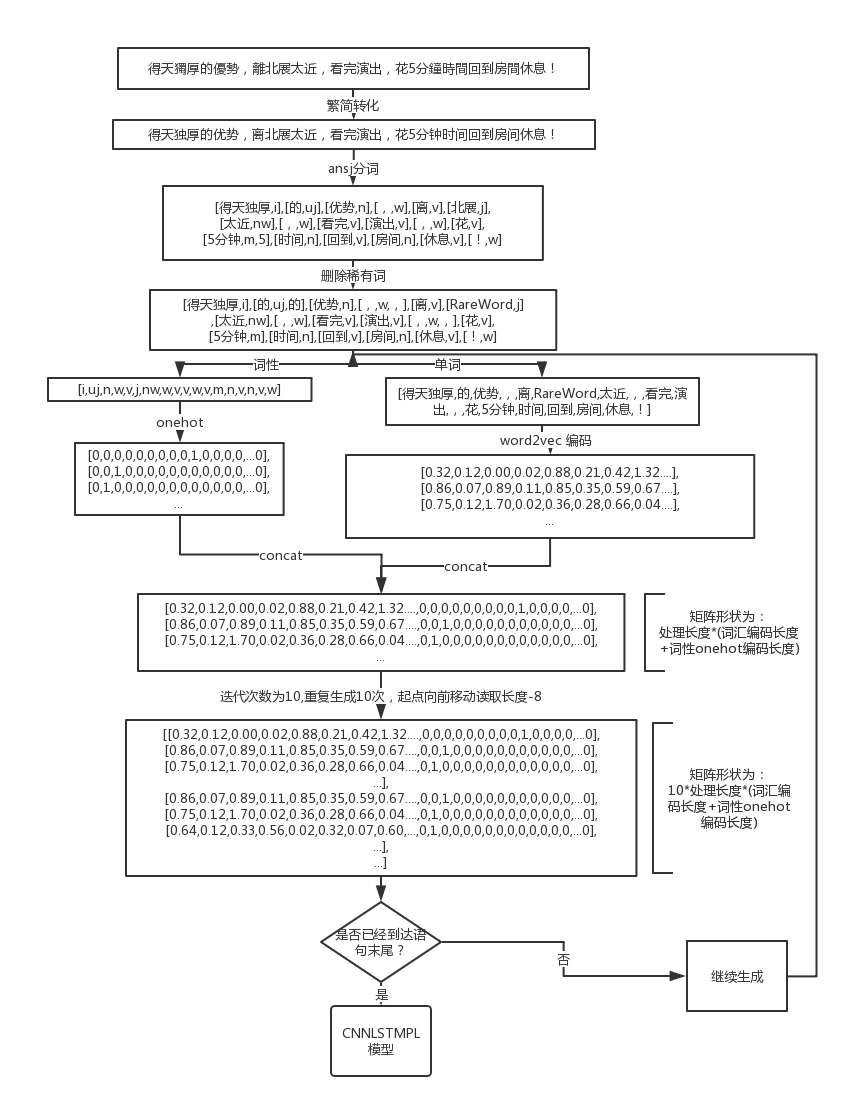
\includegraphics[width=\textwidth]{graphic/preprocessrzh.png}
\caption{CNNLSTMPL模型中文特征生成流程图 \label{fig:preprocessrzh}}
\end{center}
\end{figure}


\begin{figure}[!htbp]
\begin{center}
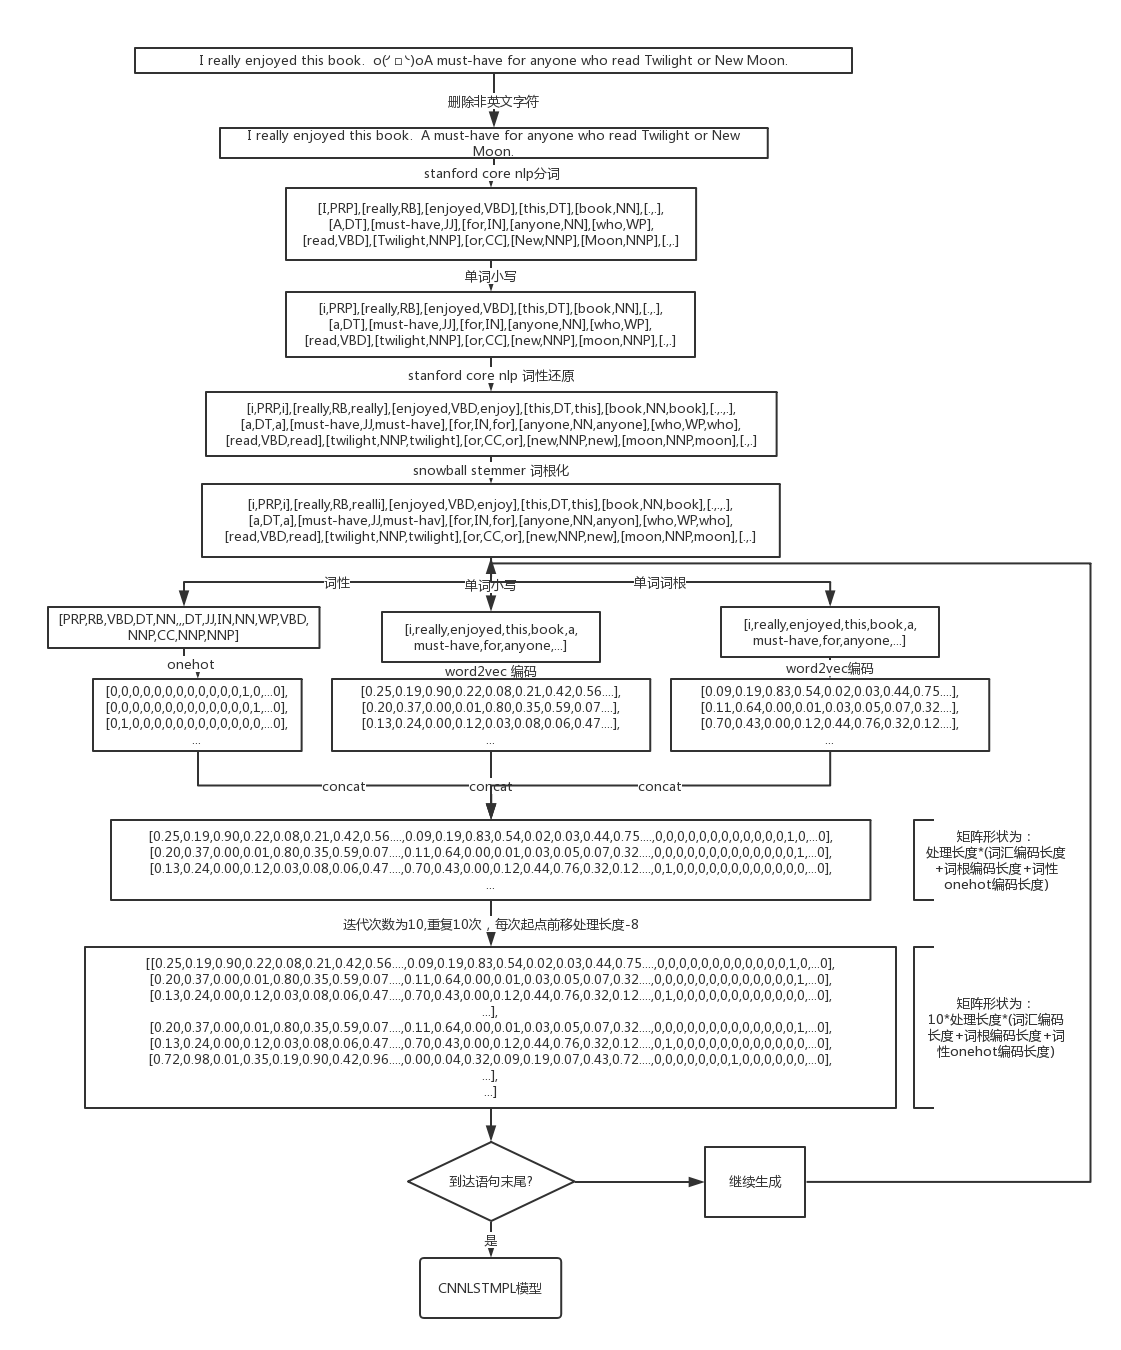
\includegraphics[width=\textwidth]{graphic/preprocessren.png}
\caption{CNNLSTMPL模型英文特征生成流程图 \label{fig:preprocessren}}
\end{center}
\end{figure}